\documentclass[dvipdfmx]{article}
\usepackage{tikz}

\begin{document}
  \begin{minipage}{0.33\hsize}
   \begin{center}
    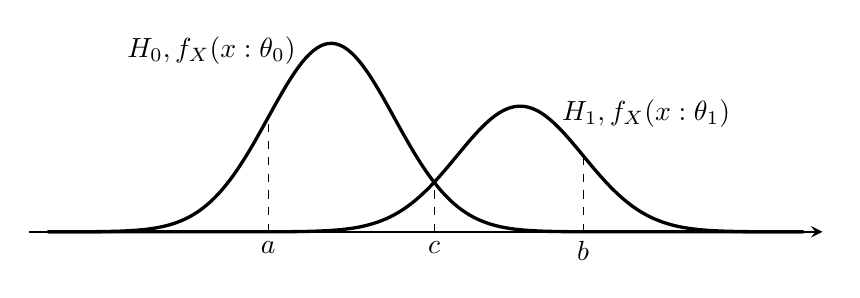
\begin{tikzpicture} [xscale = 0.8, yscale = 4]
      % 座標軸
      \draw [thick, -stealth](-6.3,0)--(6.3,0) node [anchor=north]{$$};

      % 正規分布
      \draw [very thick, domain=-6:6, samples=200] plot(\x, {1.5*exp((-(\x+1.5)^2)/2)/(sqrt(2*pi))});
      \draw [very thick, domain=-6:6, samples=200] plot(\x, {exp((-(\x-1.5)^2)/2)/(sqrt(2*pi))});

      % 補助線
      \draw [dashed](-2.5,0) node [anchor=north]{$a$} -- (-2.5,{1.5*exp((-(-2.5+1.5)^2)/2)/(sqrt(2*pi))});
      \draw [dashed](0.135,0) node [anchor=north]{$c$} -- (0.135,{exp((-(0.135-1.5)^2)/2)/(sqrt(2*pi))});
      \draw [dashed](2.5,0) node [anchor=north]{$b$} -- (2.5,{exp((-(1.0)^2)/2)/(sqrt(2*pi))});

      % 説明
      \node [anchor=south] at (-3.4, 0.5) {$H_0,f_X(x:\theta_0)$};
      \node [anchor=south] at (3.5, 0.3) {$H_1,f_X(x:\theta_1)$};
    \end{tikzpicture}
   \end{center}
  \end{minipage}
\end{document}